\section{Artefact Development Report}
\label{Minimum Artefact section}
\todo{Change this section to include T2 works}
In this section, we describe the progress on the artefact development, the detail and context for the experiments are given as Section \ref{Research Design section}.
We address the process (see Section \ref{Research Activities section}) by implementing a series of exploratory experiments.
The artefact is a Python notebook file containing Python scripts to run the experiment.
We run the notebook with IBM Quantum Experience, as it provides online services for running and simulating quantum hardware.
We use the hardware noise sample from the device \emph{ibm\_perth} to configure our simulator to achieve a most accurate to that of a real quantum neural network training scenario.

We have chosen the ansatz \emph{Real Amplitude} and a custom ansatz (see Section \ref{Sec: Creating Ansatzes}) as the objects of study.
The four treatments applied to these ansatzes are further discussed in Section \ref{Sec: Treatments for ansatzes} (see Table \ref{implementation of methods table} and Figure \ref{Research Activities Figure}).
\almarginpar{Need to update this table, or make another one to include the classification problem}
We summarise the experiment results from Section \ref{Result section} in Table \ref{Tab: Experiment Phase 1 Res} and \ref{Tab: Experiment Phase 2 Res}.



\subsection{The Quantum Provider}
For this experiment, we are using the quantum emulator provided by Qiskit.
The QASM simulator is used to mimic an IBMQ device.
Additionally, the QASM simulator, by default, has no noise, so we can expect the result to be noise-free.
Note that the fault-free emulators do not reflect quantum devices precisely as the actual devices may suffer from various types of noise.
However, considering the allowed time span for these experiments, we will use the QASM simulator for T1-2022 and leave the actual quantum devices for future works.

\subsection{Creating Ansatzes}
\almarginpar{Which of the ansatze would be most useful to support QNN? Wouldn't RealAmplitudes be useful for "real" QNN implementation?}
We have chosen the \textit{NLocal} and \textit{TwoLocal} classes from the Qiskit circuit library to explore the two ansatzes structures

An example of circuits generated by Qiskit is visualised in Figure \ref{Ansatz samples}.
By altering the repetition number and qubit number, we can generate different ansatz.
The circuit depth is the largest number of gate operations across all qubit registers in a circuit.
Furthermore, as the circuit high-level definition is translated into the gate set available on a given quantum machine, the circuit depth may significantly increase.
Obviously, as the ansatz repetition grows, the circuit depth also grows.
Figure \ref{Ansatz samples} further shows that for a fully entangled ansatz, the higher number of qubits also leads to deeper circuit.

\begin{figure}
    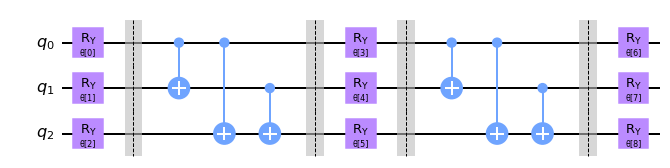
\includegraphics[width=\textwidth]{Artefact/Appendices/ansatz3-2.png}
    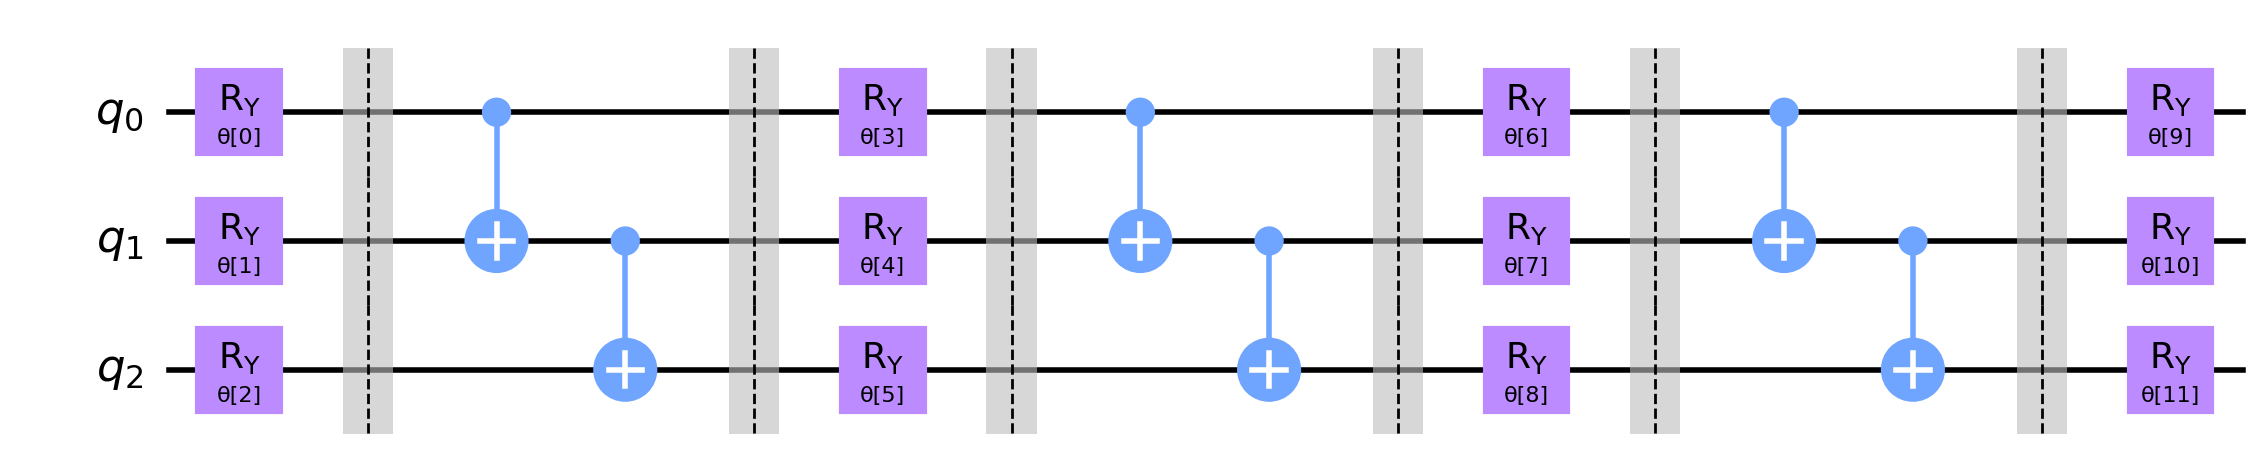
\includegraphics[width=\textwidth]{Artefact/Appendices/ansatz3-3.png}
    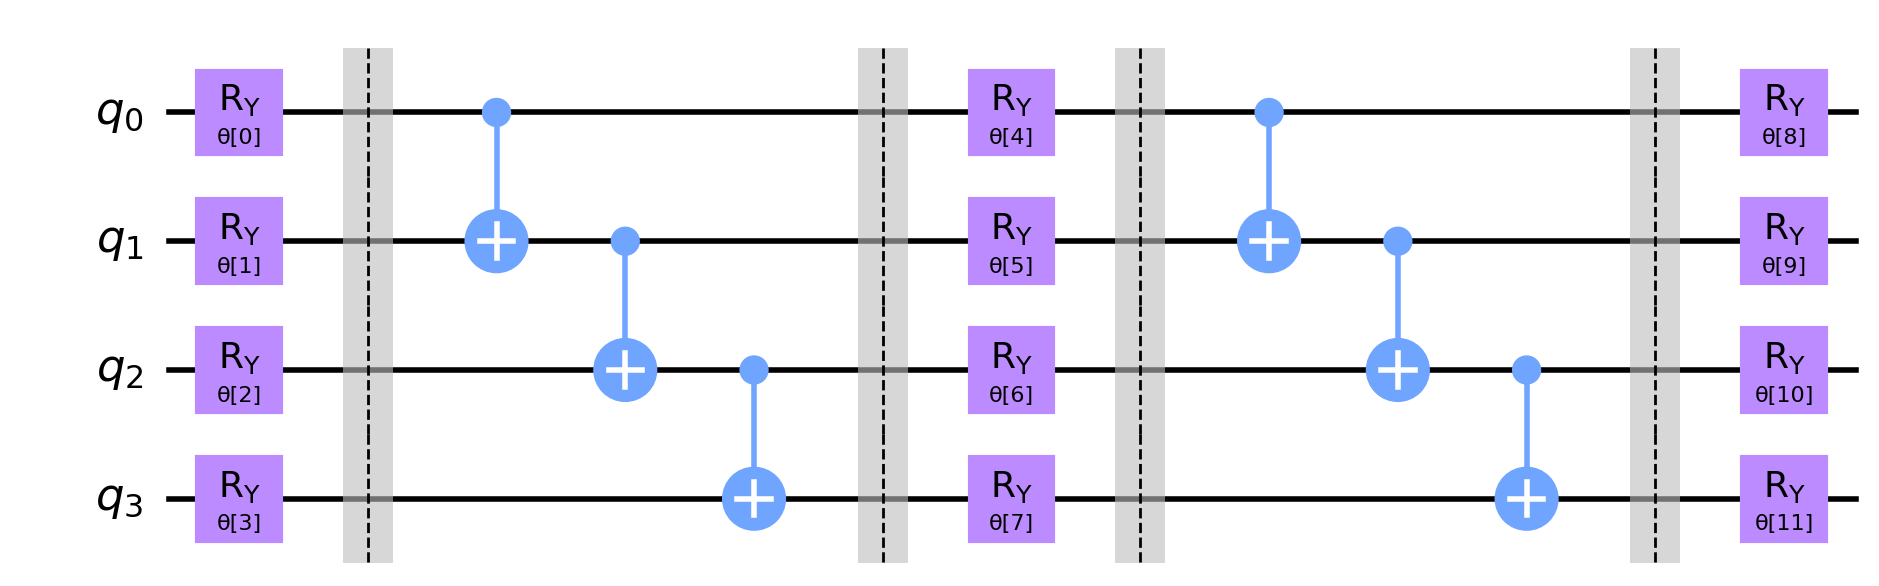
\includegraphics[width=\textwidth]{Artefact/Appendices/ansatz4-2.png}
    \caption{
        Samples of parameterised circuits generated by the Qiskit framework with 'full entanglement' option.
        The ansatz is a sequence of rotation layers and entanglement layers.
        Above: an ansatz of three qubits and two repetition layers.
        Middle: an ansatz of three qubits and three repetition layers.
        Below: an ansatz of four qubits and two repetition layers.
    }
    \label{Ansatz samples}
\end{figure}

\subsection{Treatments for ansatzes} \label{Sec: Treatments for ansatzes}
\todo{add method 2 and 3}
We apply the methods in Section \ref{Research Design section} to the ansatzes as described in section \ref{Sec: Creating Ansatzes}.

\subsubsection{Method \#0: Unrestricted} \label{Sec: Method0}
As discussed in the Section \ref{Research Design section}, the goal of this configuration is to produce a general multilayered perceptron network without any restriction.
The ansatzes will have unrestricted growth of circuit depth with a global cost function.
The initial parameters of this ansatz are randomised.
We implement the default ansatz to have the number of qubits and repetition increased iteratively.

\subsubsection{Method \#1: Local Cost Function and Shallow Depth Implementation} \label{Sec: Method1}
We implemented the \textit{Global Cost Function} as the measurement output for all qubits, while the \textit{Local Cost Function} is the measurement for the first two qubits.
Section \ref{Shallow Circuits, Local Cost Function section} and figure \ref{cost functions} previously explained the differences between the two cost functions.
The shallow ansatz is the same as the default.
However, the repetition number is kept as a constant number.

\subsubsection{Method \#2: Layerwise Learning} \label{Sec: Method2}
The ansatses will have unrestricted growth of circuit depth, and a measurement gate for each qubit at the end as the global cost function.
While the construction process is similar to that of the method \#0, we follow the \emph{Layerwise learning} algorithm as described in Section \ref{Sec: Layerwise Learning} to obtain the optimal initial parameters.

\subsubsection{Method \#3: Identity Blocks} \label{Sec: Method3}
For this method, we create a custom ansatz as an identity block.
As discussed in Section \ref{Sec: Identity blocks}, one identity block has two part, the first part can have its parameter randomised, while the second part invert the first part.
Figure \ref{Fig: Identity Ansatz Sample} demonstrate an identity block with two qubits.
For the first part of the identity block, we use the Real amplitudes with one repetition layer plus one rotation layer.
The gates of this part has their parameters randomised.
The second part of the identity block simply reverse the sequence of rotation layers and entanglement layers.
The gates of this part has their parameters chosen as invert of the first layer.
\begin{figure}
    \centering
    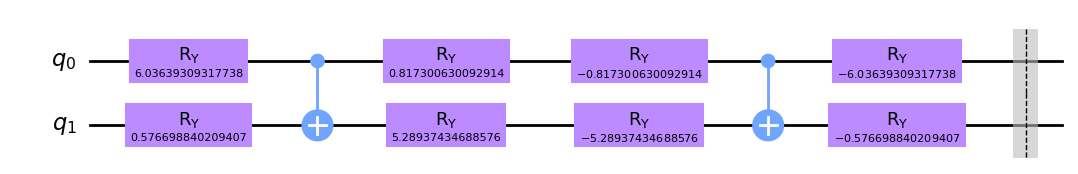
\includegraphics[width=\textwidth]{Artefact/Appendices/ansatz-identity.png}
    \caption{An Identity Block of two qubits, the first part has four random parameters, the second part is an invert of the first part.}
    \label{Fig: Identity Ansatz Sample}
\end{figure}


\subsection{Visualise the Variance} \label{Sec: Visualise the Variance}
\todo{move to design section}
We use the parameter shift rule from Eq. (\ref{Parameter-shift rules}) as implemented in the Qiskit Gradient library to calculate the gradient variance.
The BP phenomena can be verified when the gradient variance exponentially decreases with an increased number of qubits and repetition layers.

To visualise the gradient variances, we have plotted a range of random parameters for each ansatz as the initial starting point.
Such randomised parameters are generated 100 times uniformly to calculate the gradients.
We then plot the variance values of the gradients for different numbers of qubits and repetition values for a range of 2 to 7 qubits and ansatz layer repetition.
Note that the neural network generated in this experiment is not designed to answer a problem.
We will focus on the trainability of each method in the later phase of the experiment.

In short, we use 100 uniformly randomised parameters to scan the gradient.
Then we calculate the "slope" of the gradient.

\subsection{Classification Problem} \label{Sec: Classification Problem}
We implement a variational quantum classifier as previously discussed in the section \ref{VQA}.
The algorithm includes two stages: a training stage and a classification stage.
We use a dataset generated by Qiskit machine learning package for the algorithm.
The data was also used for a classification algorithm by Havlíček et al. \cite{havlicekSupervisedLearningQuantumenhanced2019}.

The quantum circuit for both stages is constructed from three parts: the feature map to encode data, the ansatz to perform optimisation and finally, a final rotation layer for measurement (see Figure \ref{Fig: Quantum circuit for classifier}).
The number of features will dictiate the number of qubits, in out case, we will be using two qubits for the quantum circuit.
For the method \#0 and \#2, there is no restriction on ansatz depth, so we build the ansatz to have 7 repetitions (15 depth units).
For the method \#1 with restriction for ansatz depth, we only use 2 reptitions (5 depth units).
For the customised ansatz in method \#3, we construct the ansatz to have the depth closer to that of method \#1 and \#2. We will be using three identity blocks as the ansatz, which results in 18 depth units.

The dataset consited of 50 labeled datapoints with two features is used for the traning stage.
The quantum circuit will be estimated as required by Gradient Descent algorithm provided by Qiskit to optimise the ansatz parameters.
For the classification satge, we use another set of 20 datapoints, and run the classifier with the optimised parameters obtained from the training stage.
The classifier would produce the predicted labels for each testing datapoint.
Then, we compare these predicted labels to the actual provided labels.

We collect the optimizer history (loss function per iteration) by implement a callback function for Gradient Descent algorithm.
The score $s$ of the classifier is calculate as the percentage likeliness of the predicted labels array compared to the actual labels array:
\begin{equation}
    s = 100\% (1 - \text{MSE})
\end{equation}
for $\text{MSE}$ is the mean square error of the actual labels array $Z$ and predicted labels array $\hat{Z}$ of length $n$:
\begin{equation}
    \text{MSE} = \frac{1}{n}\sum^n_{i=1}(Z_i - \hat{Z}_i)^2,
\end{equation}



\begin{figure}
    \centerline{
    \Qcircuit @C=1em @R=2em {
    \lstick{\ket{0}} & \multigate{1}{U_{\phi}(\vec{x})}    & \multigate{1}{W(\vec{\theta})}    & \meter & \rstick{z_1} \cw \\
    \lstick{\ket{0}} & \ghost{U_{\phi}(\vec{x})}           & \ghost{W(\vec{\theta})}           & \meter & \rstick{z_n} \cw \\
    }
    }
    \caption{
        Quantum Variational Classifier implemented for the experiment.
        The initial qubit state $\ket{0}^n$ is applied with a feature map $U_{\phi}(\vec{x})$ to encode data $\vec{x}$ from our dataset.
        Then, an unitary operation $W(\vec{\theta})$ is applied as the ansatz, follow up with a measurement layer.
        The output string $z \in \{0,1\}^n$ is mapped as label for the given datapoint $\vec{x}$.
    }
    \label{Fig: Quantum circuit for classifier}
\end{figure}


\subsection{Results and Analysis} \label{Result section}

\subsubsection{Sampling Gradients results}
\begin{table*}
    \centering
    \begin{tabular}{|| l l l ||}
        \hline
        \textbf{Ansatz} & \textbf{Method}                         & \textbf{Variance exponential fit} \\[0.5ex]
        \hline \hline
        Real Amplitude  & \#0: No restriction                     & -0.63                             \\
        Real Amplitude  & \#1: Local Cost function, shallow depth & -0.06                             \\
        Real Amplitude  & \#2: Layerwise Learning                 & -0.57                             \\
        Customised      & \#3: Identity Blocks                    & -0.60                             \\
        \hline
    \end{tabular}
    \caption{
        The phase one of the experiments that we implemented in the Python Notebook.
        We test the same ansatzes with different methods, we record the results as the vanishing rate of gradient when the number of qubits increased.
        The differences between the \emph{fit} values are small.
        However, consider the unit measure is \emph{exponential} (i.e. $10^{-1}, 10^{-2}$) the growth or decay rates can be significant.
    }
    \label{Tab: Experiment Phase 1 Res}
\end{table*}

Table \ref{Tab: Experiment Phase 1 Res} states all the combinations of ansatzes and methods.

The ansatz gradient variances decay as expected for the unrestricted setting.
The decay rate is exponentially fitted with the rate of -0.63.
The figure \ref{Plot ansatzes variance}a shows the results of the ansatz in this configuration.
The semi-log plots portray the variances of gradient from the ansatz in the unrestricted configuration.
Consider that the unit measure for variance is in \emph{exponential} form, so the linear graph is exponentially closer to zero for each qubit added to the circuit.
This result indicates that the cost function landscape becomes flatter and flatter.
Eventually, the gradient would reach a near-zero value across a large plateau, which would be inefficient for any gradient-based optimization algorithm to train the model.
We discussed this phenomenon in Section \ref{Barren Plateaus section}.

\todo{changing the number to actual name}
\begin{figure}
    \centering
    \begin{subfigure}[b]{.49\linewidth}
        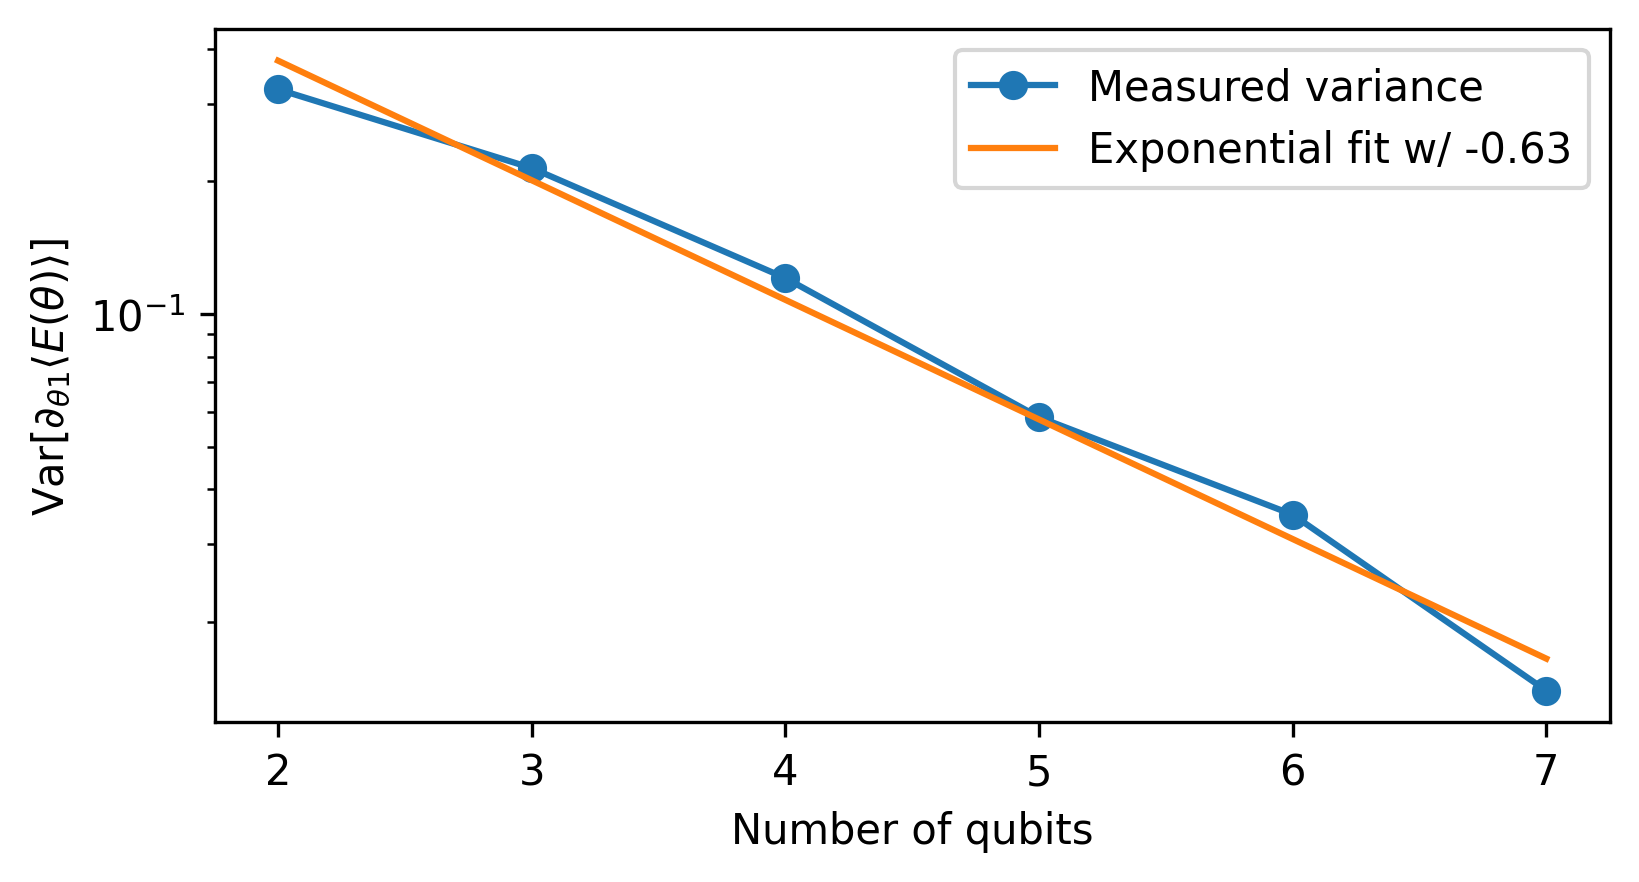
\includegraphics[width=\linewidth]{Artefact/Appendices/var0.png}
        \centerline{0) Default method}
    \end{subfigure}
    \hfill
    \begin{subfigure}[b]{.49\linewidth}
        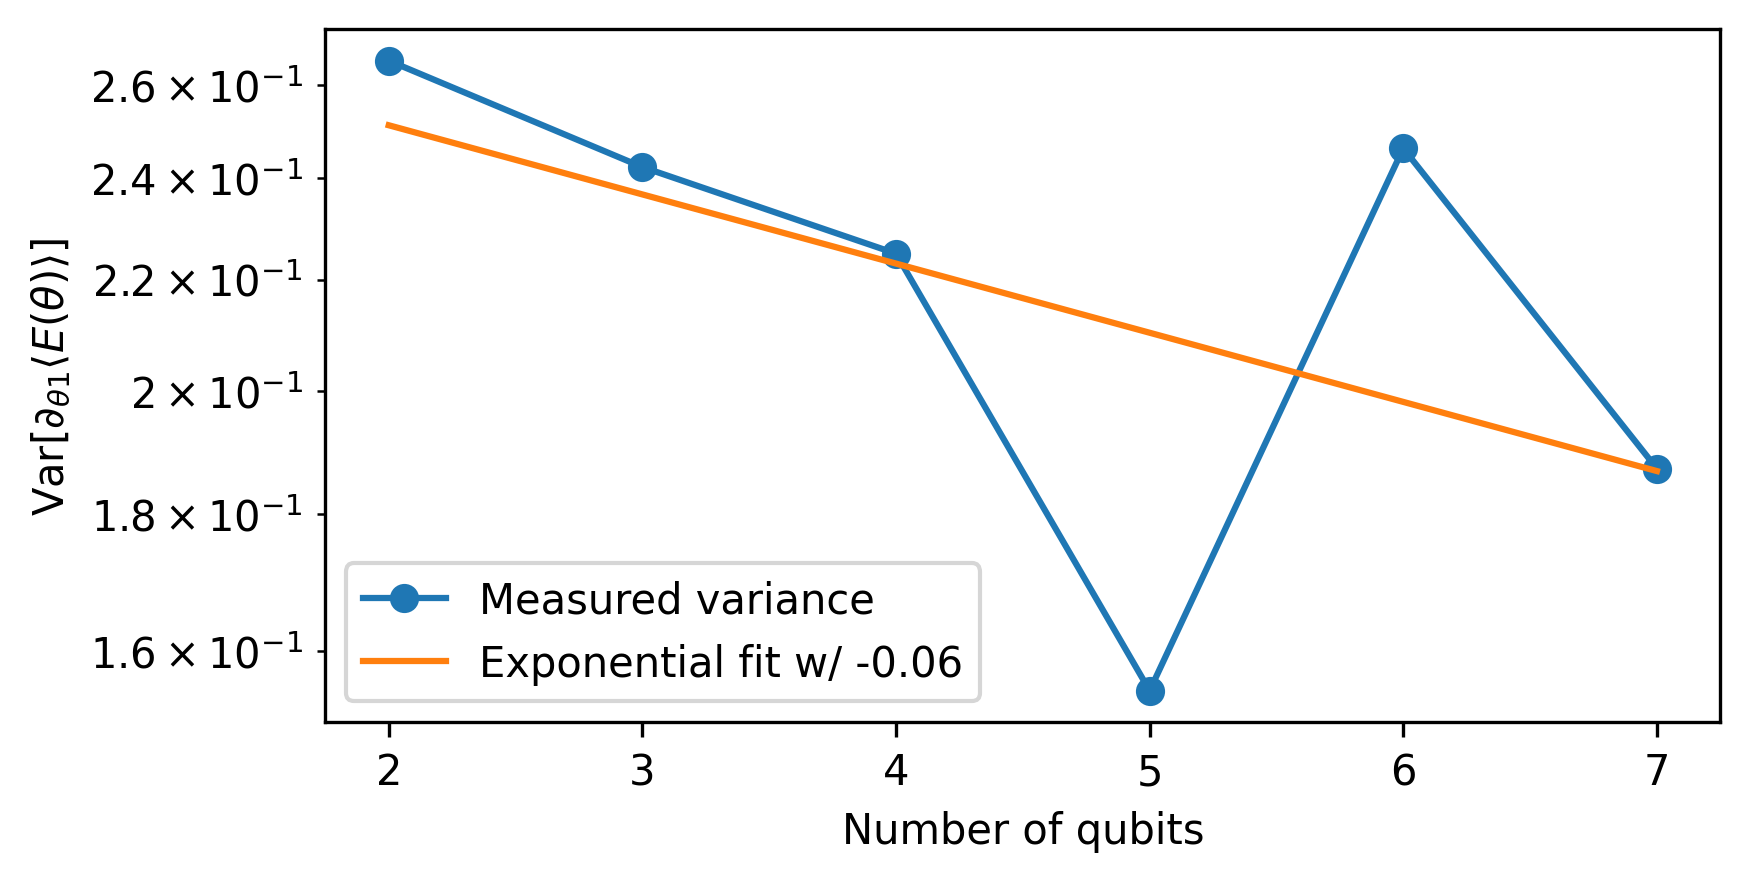
\includegraphics[width=\linewidth]{Artefact/Appendices/var1.png}
        \centerline{1) Shallow circuit and local cost function}
    \end{subfigure}

    \begin{subfigure}[b]{.49\linewidth}
        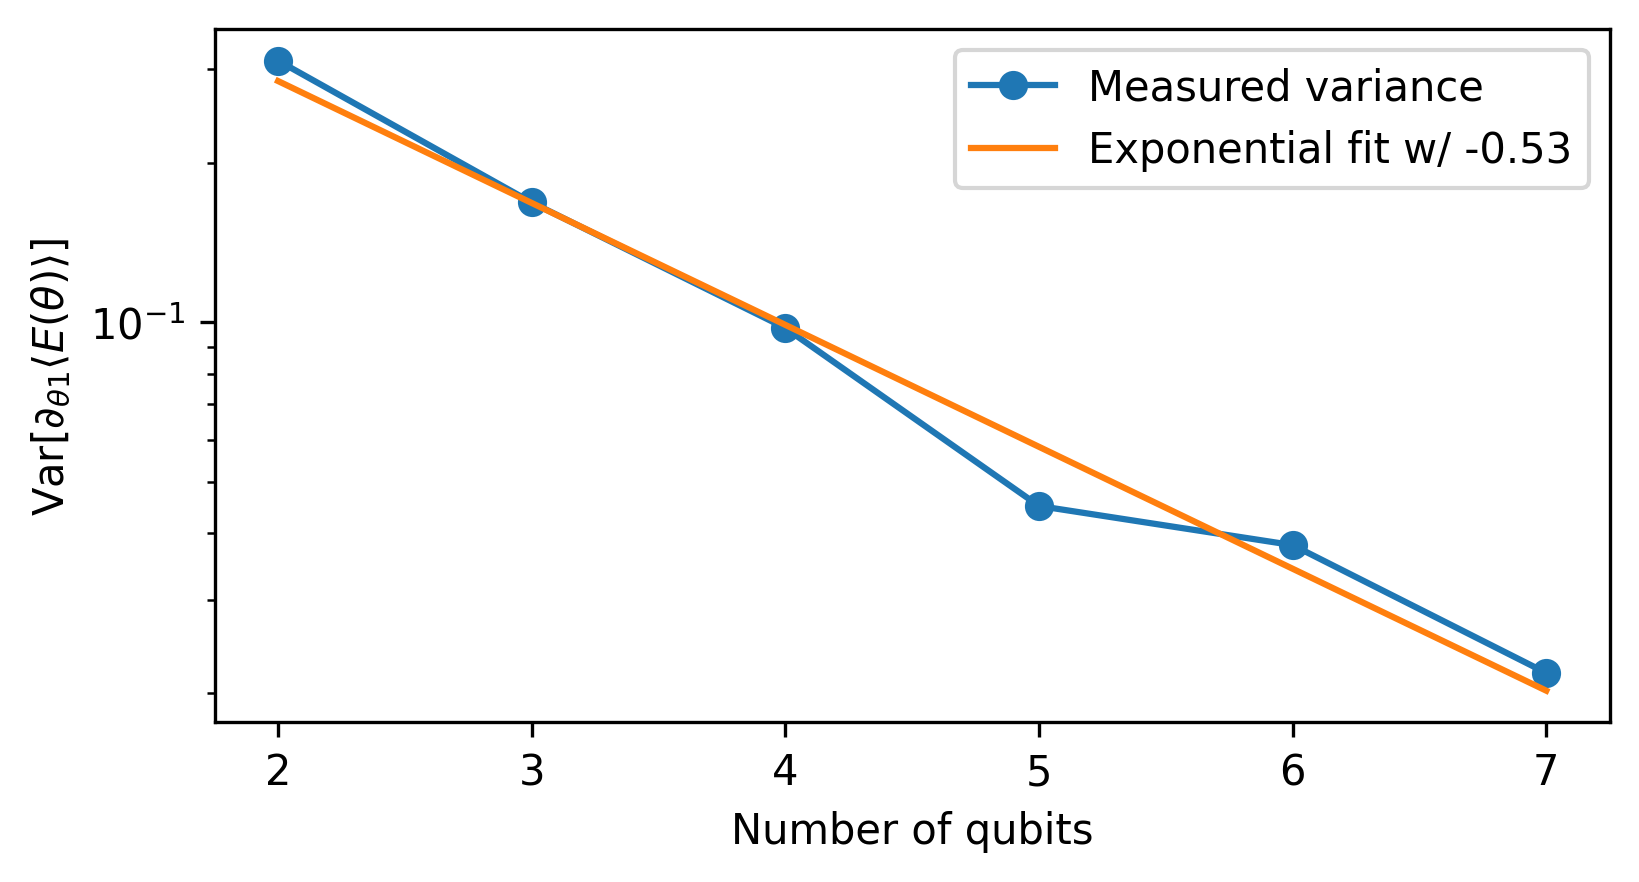
\includegraphics[width=\linewidth]{Artefact/Appendices/var2.png}
        \centerline{2) Layerwise learning}
    \end{subfigure}
    \hfill
    \begin{subfigure}[b]{.49\linewidth}
        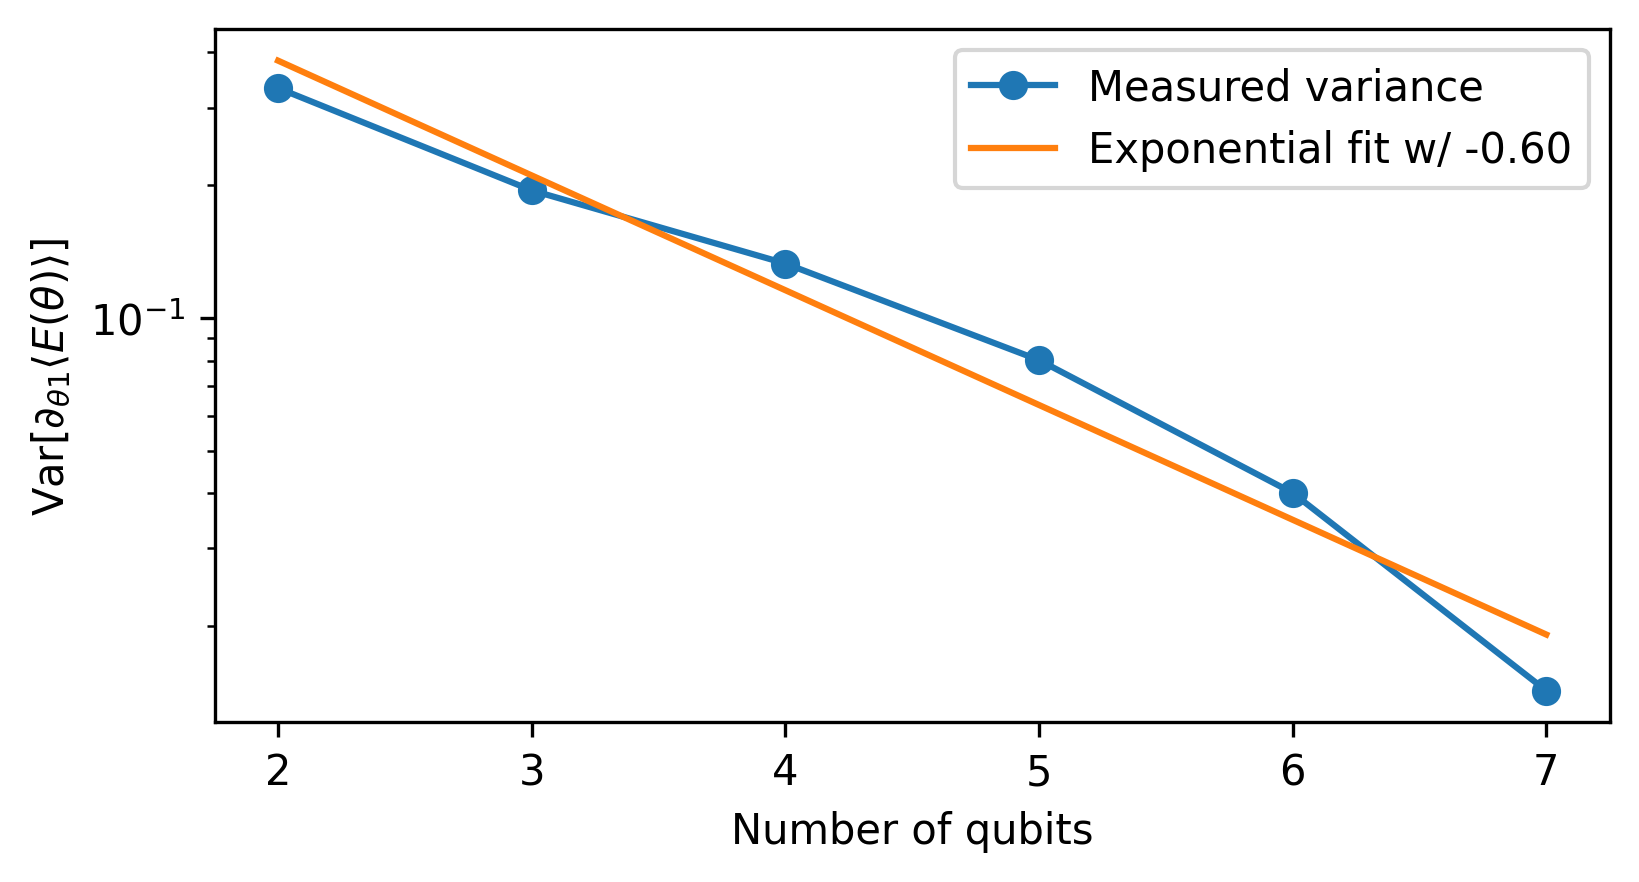
\includegraphics[width=\linewidth]{Artefact/Appendices/var3.png}
        \centerline{3) Identity blocks}
    \end{subfigure}

    \caption{
        The variances of gradient from differences ansatzes in the four configurations.
        For each iteration, we increase the qubit and repetition count by 1, starting from 2 to 7.
        The variances vanish exponentially to the number of qubits.
        For the shallow circuit - local cost function, we keep the repetition value fixed as 1 and only measure two qubits.
    }
    \label{Plot ansatzes variance}
\end{figure}

In contrast, for the case of Local Cost Function and Shallow circuit, we observe that the variances of the ansatz' gradient did not vanish when we attempted to increase the number of qubits.
The slope of the ansatz in this case decay exponentially fit with -0.06.
This implies that the cost function landscape can sustain the slope.
Figure \ref{Plot ansatzes variance}b shows the result of the experiment for local cost function and shallow circuit.
We can see that the ansatz produced an unstable graph which mean the trainability of gradient-based optimization algorithms would not be consistent.
For example, the variance value for 6 qubits is higher compared to 3, 4 or 5 qubits.

To compare the effectiveness of the different treatments, we plot the variance graph of above mention cases in Figure \ref{Fig: Plot Variances} and the Table \ref{Tab: Experiment Phase 1 Res}.
The results have shown the differences in the decay rates of different ansatzes and methods.
Overall, the ansatzes with the local cost function and restriction on circuit depth have their variance values remaining higher and being more consistent for higher qubit count.
The ansatz with this treatment, therefore would not possess a barren plateau.
On the other hand, the values for the other cases shrink exponentially and eventually, the near-zero gradient around the initial point will expand to a large plateau.


\begin{figure}
    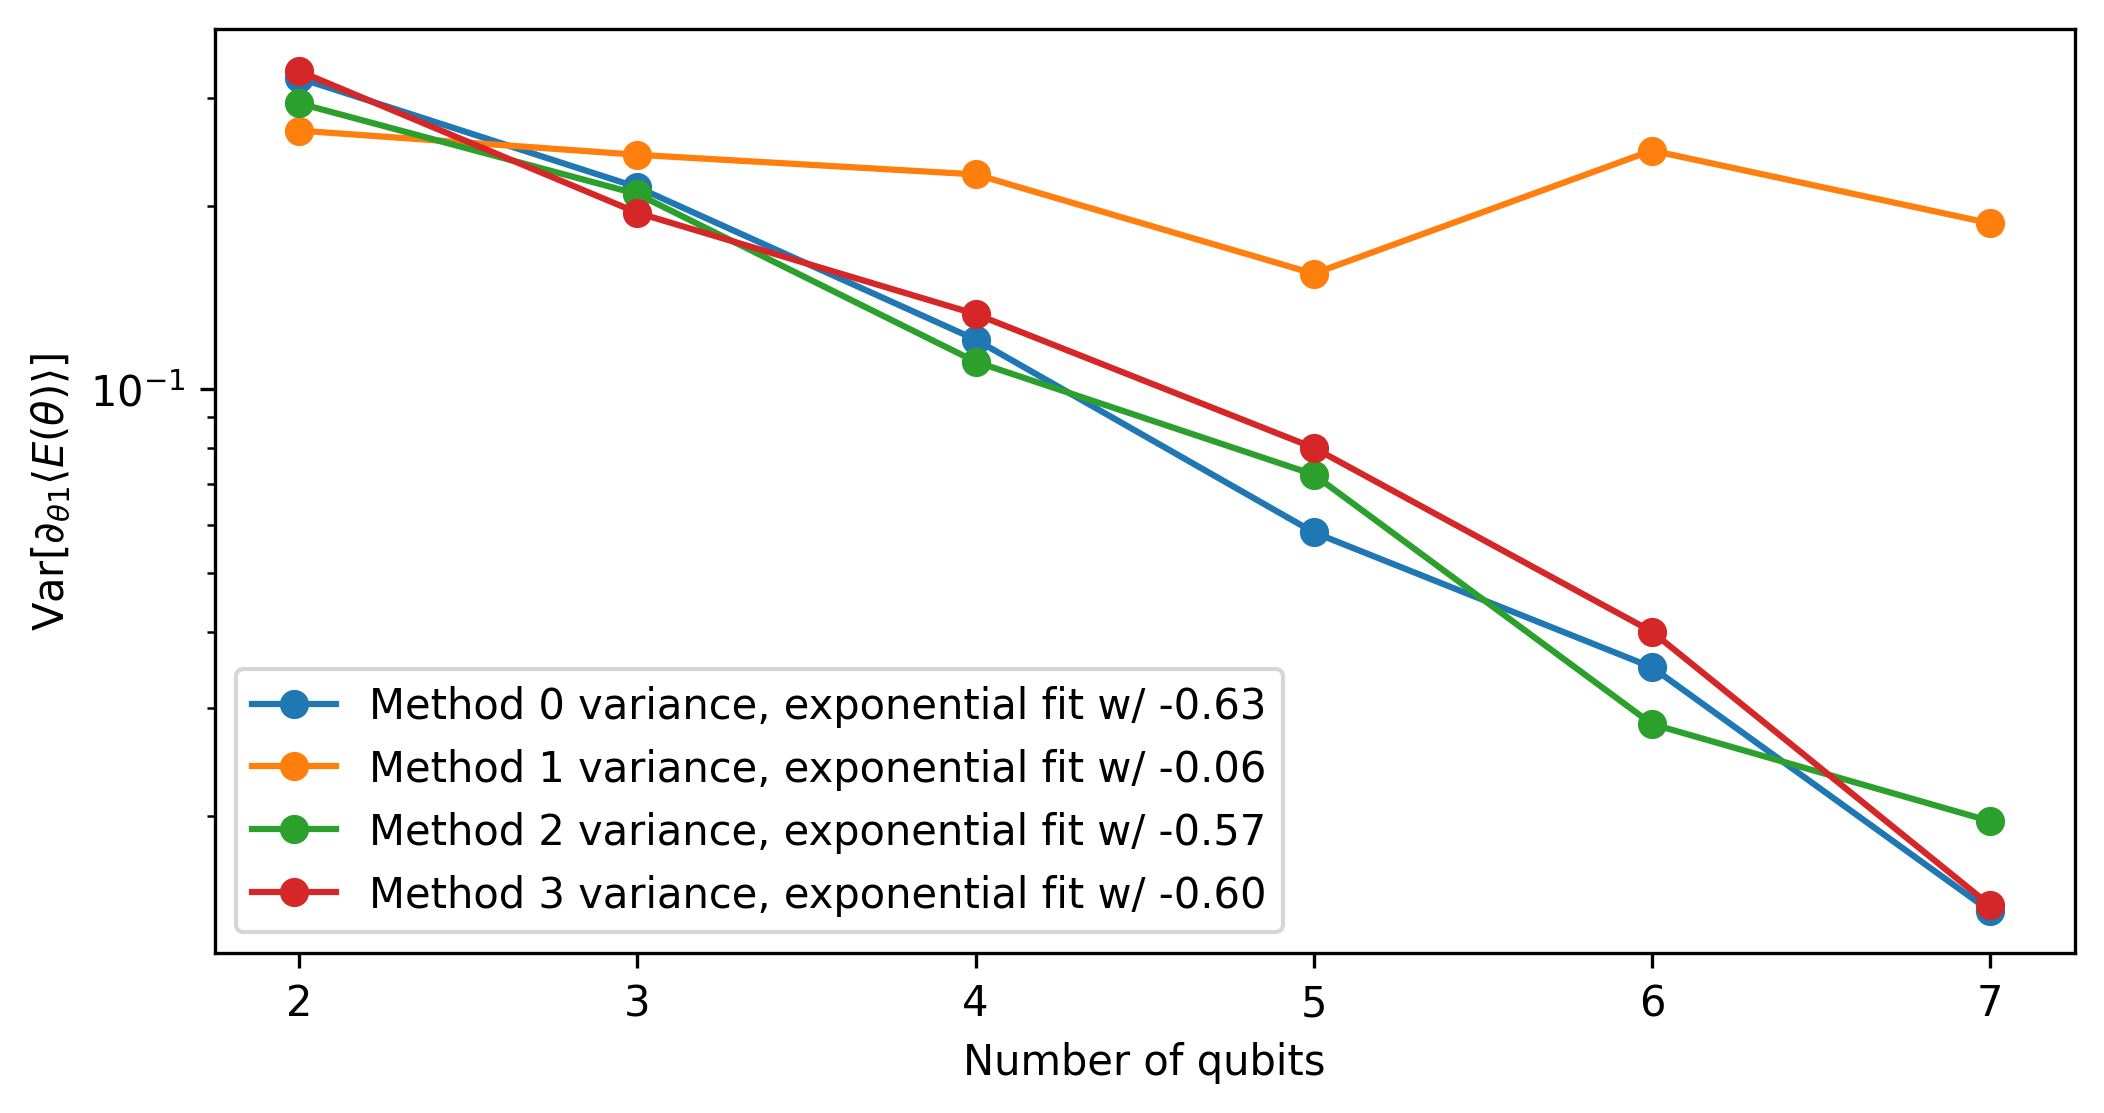
\includegraphics[width=\linewidth]{Artefact/Appendices/variances.png}
    \caption{
        Comparison of the variance values of the ansatzes with four treatments applies.
        The ansatz with local cost function and fixed depth has its variance decay at a significantly smaller rate (-0.06) compared to the rest.
    }
    \label{Fig: Plot Variances}
\end{figure}


\subsubsection{Classification Results}

\begin{table*}
    \centering
    \begin{tabular}{|| p{4cm} p{2cm} p{2cm} p{2cm} p{2cm} ||}
        \hline
        \textbf{Method}                          & \textbf{Circuit depth} & \textbf{Parameters count} & \textbf{Minimum loss} & \textbf{Score} \\
        \hline \hline
        0: No Restriction                        & 15                     & 16                        & 0.57                  & 72.50\%        \\
        1: Local Cost Function - Shallow circuit & 5                      & 6                         & 0.57                  & 80\%           \\
        2: Layerwise Learning                    & 15                     & 16                        & 0.39                  & 92.5\%         \\
        3: Identity Blocks                       & 18                     & 24                        & 0.39                  & 90\%           \\
        \hline
    \end{tabular}
    \caption{
        The result as recorded from the phase two of the experiment.
        We use the ansatzes from four methods as the neural network to solve a classification problem.
    }
    \label{Tab: Experiment Phase 2 Res}
\end{table*}

The unrestricted and local cost function - shallow depth ansatzes loss functions both converged at a value of 0.57.
However, we can see that the local cost function and shallow circuit ansatz achieved higher accuracy in the classification test (at 80\% accuracy) than the unrestricted ansatz (at 72.5\% accuracy).
However, by restricting the ansatz depth, we may have limited the model capacity, this also applies to classical machine learning \cite{ianDeepLearningAdaptive2016}.
As more complex functions would require higher model capacity, thus higher layer count and qubit count, the local cost function - shallow depth method is suitable if the dataset represents a simple function.

\todo{) may have BP, but 1 does not have cap enough to learn, so it converged but still very high}

The identity blocks can achieve a similar loss value as the layerwise learning method (0.39) with a bit lower accuracy.
We can see that with the optimised initial parameters, the loss function can converge faster compared to identity blocks initialisation.
However, it would take more time to obtain the optimal initial parameter due to the training process (see Section \ref{Sec: Method2}), while it is much faster to generate parameters for identity blocks in Section \ref{Sec: Method3}.
The two methods also have their accuracy close to each other, scoring at 92\% for layerwise learning and 90\% for identity blocks.
Thus they are suitable for designing ansatzes of higher layer count to learn more complex functions.


To compare the effectiveness of different approaches, we plot the loss per iteration graph of above mention cases in Figure \ref{Fig: Plot Loss and Accuracy} and Table \ref{Tab: Experiment Phase 2 Res}
Overall, the methods that involve configurations on the initial parameters can achieve lower loss in training and higher score on the classification test.

\begin{figure}
    \begin{subfigure}{\linewidth}
        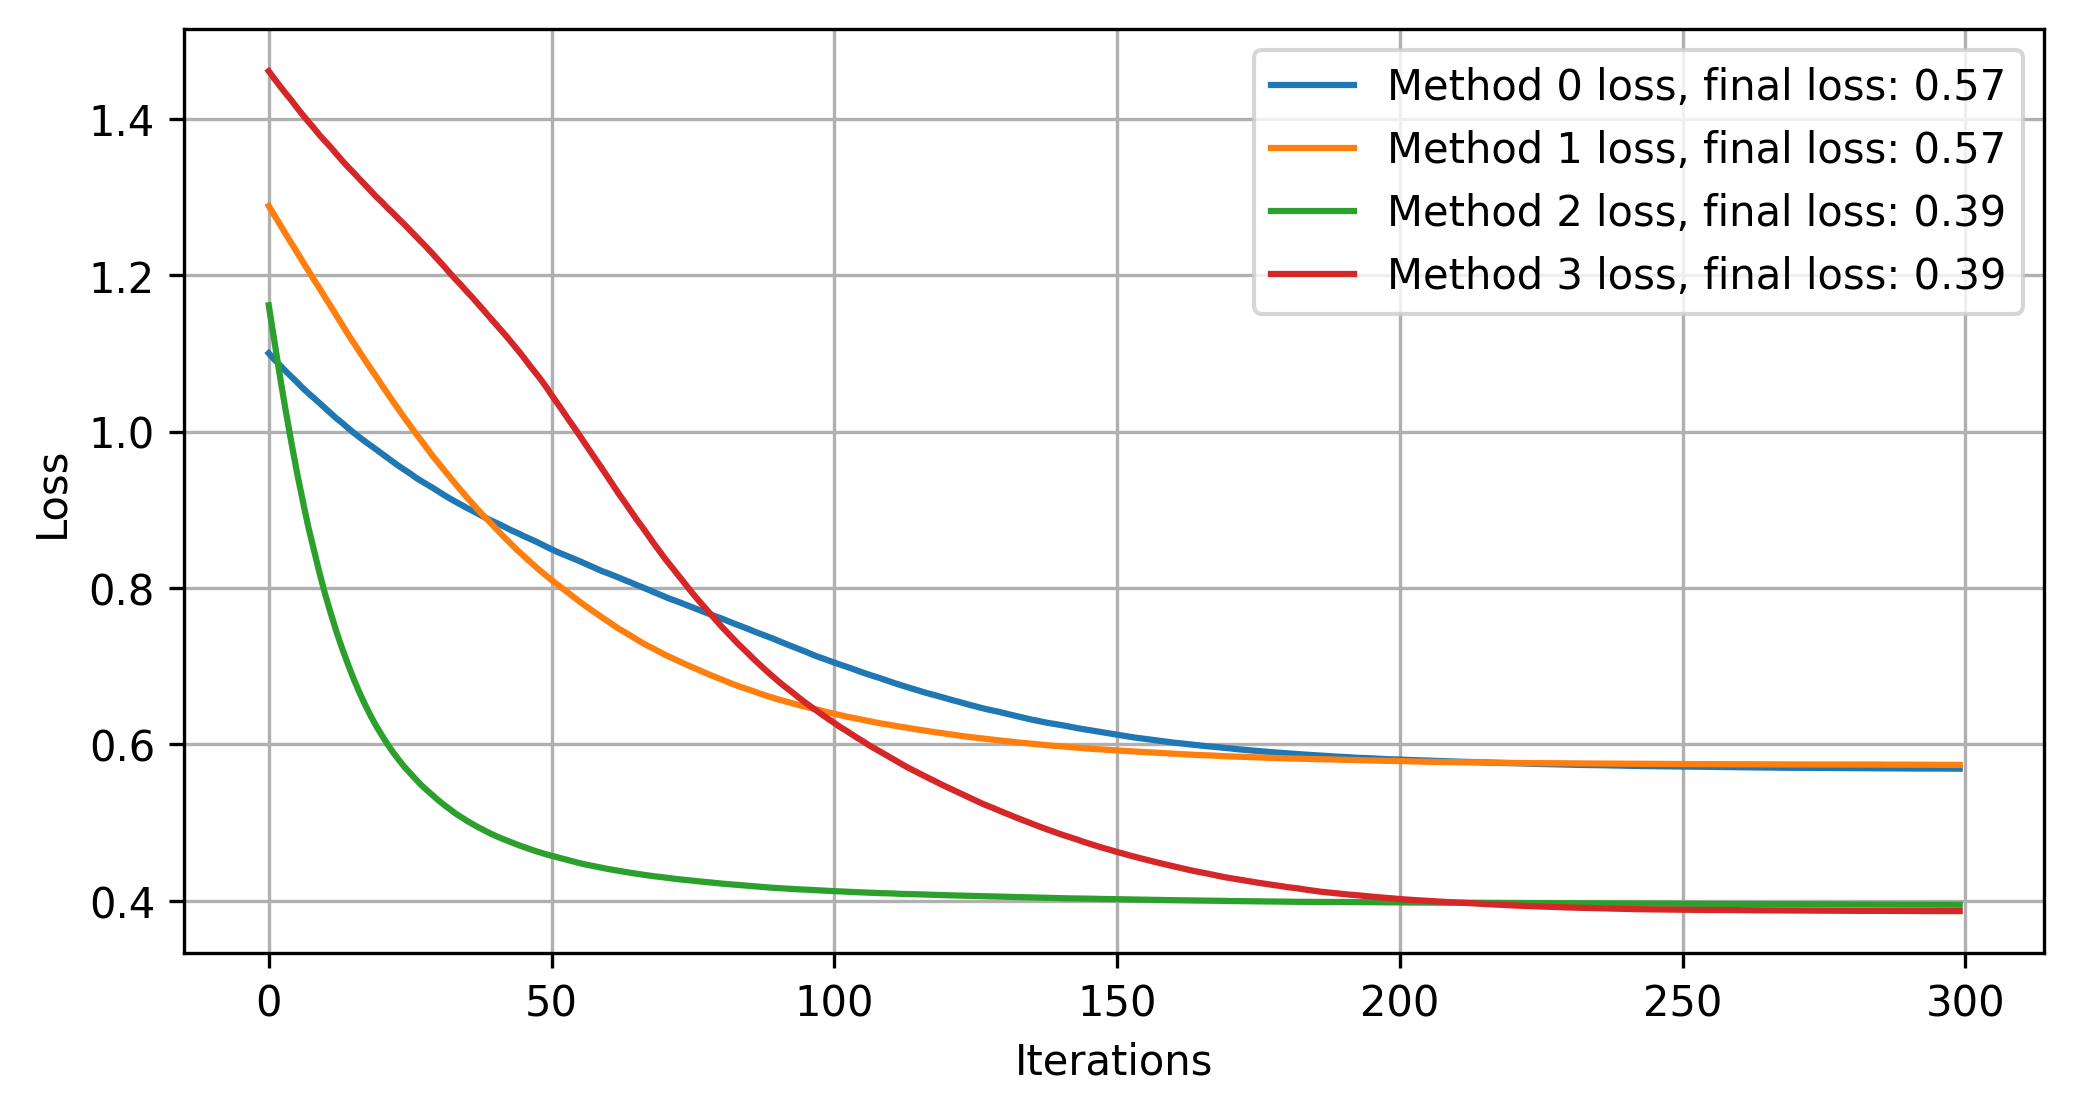
\includegraphics[width=\linewidth]{Artefact/Appendices/loss.png}
        \centerline{a) Loss function values of four classifiers in 300 steps}
    \end{subfigure}
    \begin{subfigure}{\linewidth}
        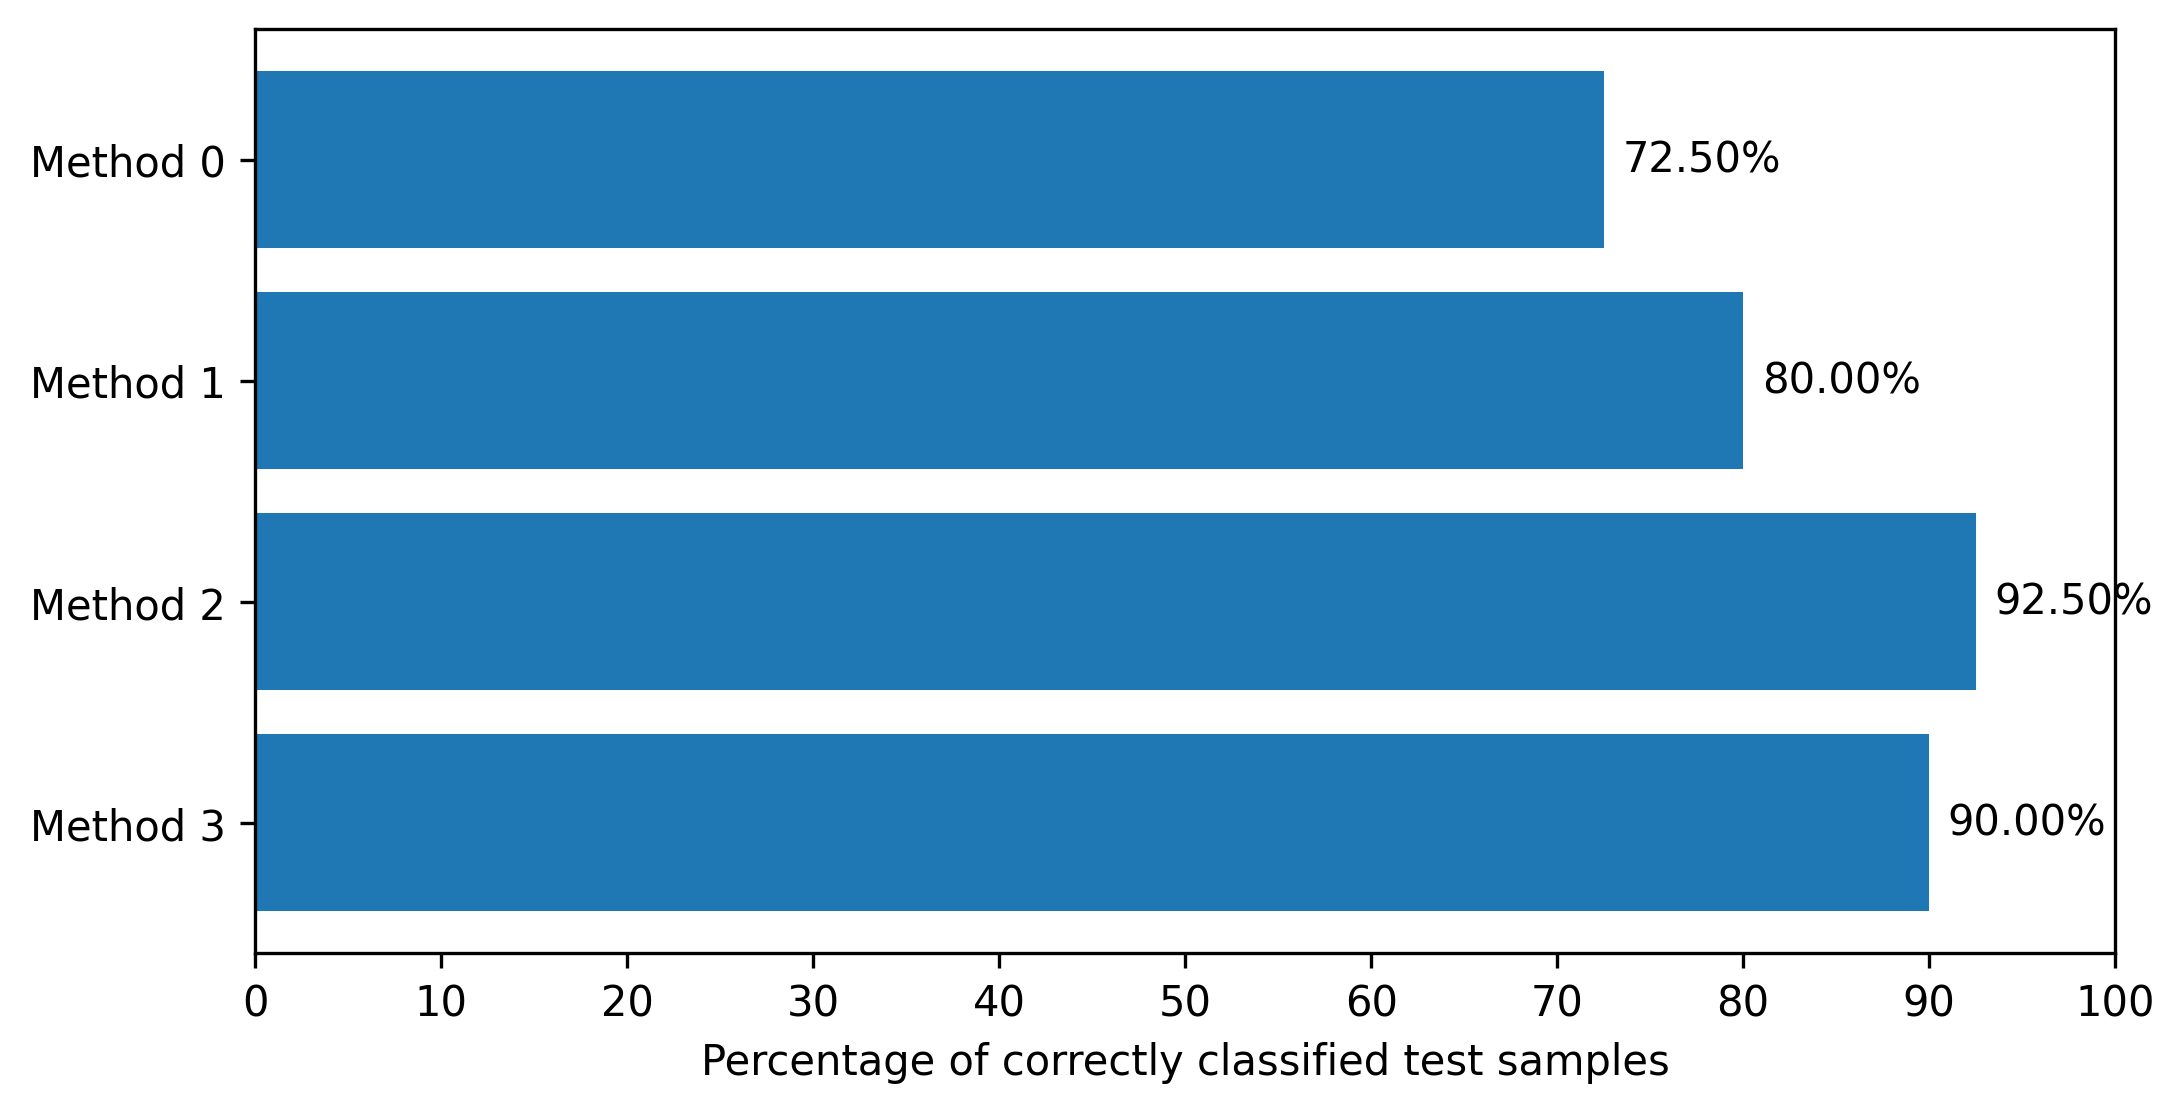
\includegraphics[width=\linewidth]{Artefact/Appendices/accuracy.png}
        \centerline{b) Accuracy score of four classifiers}
    \end{subfigure}

    \caption{
        Comparison of the loss values per iteration of gradient descent for the ansatzes with four treatments applies.
        We measure the accuracy of prediction with a set of 20 testing datapoints.
    }
    \label{Fig: Plot Loss and Accuracy}
\end{figure}


\subsection{Artefact Development Summary}

We have implemented three methods of dealing with barren plateau by altering the ansatz's depth, cost function, and initial parameters aspects.
The experiments have produced the results as the slopes of the gradients for a number of qubits, as well as the performance of ansatzes in neural network training.
The results indicate that the variances of the gradient can be stable if we set a limit on the length of the circuit and the cost function, and the training performance can increase if we carefully select the initial parameters.

With this artefact, we have addressed the research design in Section \ref{Research Design section}.
We have implemented the three methods, namely \textit{local cost function, shallow ansatz depth}, \textit{layerwise learning} and \textit{identity blocks}.
We have compared the variances in the first phase of the experiment.
We anticipate that a higher variance value does not mean the optimisation is going in the right direction, the model can still stick it in a local minimum, or the error landscape is random.
To verify the performance of these methods, in the second phase, we implemented a variational quantum neural network to solve a classification problem with a standard dataset.

The phase two of the experiments have verified that the unrestricted configuration may have run into a barren plateau, while the others can converge to their minimums - the answers.
Moreover, these experiments are conducted in an emulated environment with a noise model from \emph{ibm\_perth} backend.
Thus, this experiment can reflect the real-life situation to some extent.

According to Figure \ref{Fig: Plot Variances}, the variance values of the limited depth - cost function method at seven qubits configuration is significantly higher than the rest.
At higher qubit configuration, the barren plateaus are also more likely to appear, and the performance of these methods under this phenomenon is worth investigating.

